\documentclass[11pt,a4paper]{article}

\usepackage[utf8x]{inputenc}   % omogoča uporabo slovenskih črk kodiranih v formatu UTF-8
\usepackage[slovene]{babel}    % naloži, med drugim, slovenske delilne vzorce

\usepackage{tikz}
\usepackage{dtk-logos}
\usetikzlibrary{mindmap,shadows}



\title{Miselni vzorec za diplomo}
\author{Aljoša Rakita\\
aljo.aljo.aljo@hotmail.com\\
\ \\
Fakulteta za računalništvo in informatiko\\
Univerza v Ljubljani
\date{\today}         
}


\begin{document}
\maketitle


\begin{figure}[h]
\centering
\resizebox{\textwidth}{!}{
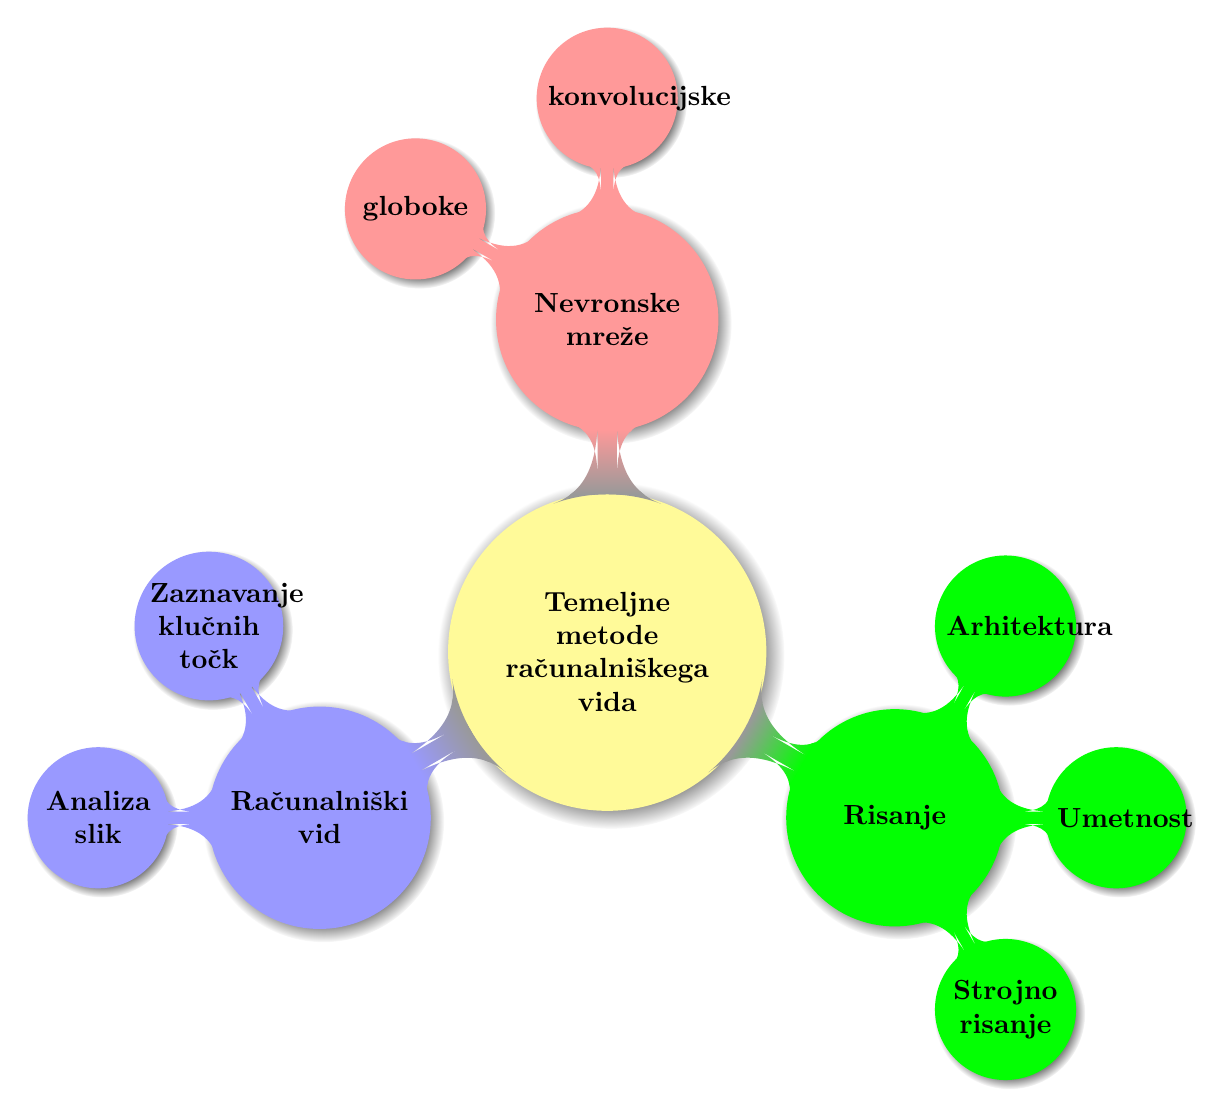
\begin{tikzpicture}[ every annotation/.style = {draw,
                     fill = white, font = \large}]
  \path[mindmap,concept color=black!40,text=black,
    every node/.style={concept,circular drop shadow},
    root/.style    = {concept color=yellow!40,
      font=\normalsize\bfseries,text width=10em},
    level 1 concept/.append style={font=\normalsize\bfseries,
      sibling angle=120,text width=7.7em,
    level distance=12em,inner sep=0pt},
    level 2 concept/.append style={font=\bfseries,level distance=8em},
  ]
  node[root] {Temeljne\\ metode\\ ra\v cunalni\v skega\\ vida} [clockwise from=-30]
    child[concept color=green!99] {
      node {Risanje} [clockwise from=60]
        child { node[concept] {Arhitektura} }
        child { node[concept] {Umetnost} }
        child { node[concept] {Strojno risanje} }
    }
    child[concept color=blue!40] {
      node[concept] {Računalniški vid}
        [clockwise from=-180]
      child { node[concept] {Analiza slik} }
      child { node[concept] {Zaznavanje klučnih točk} }
     }
    child[concept color=red!40] {
      node[concept] {Nevronske mreže}
       [clockwise from=150]
      child { node[concept] {globoke} }
      child { node[concept] {konvolucijske} }
    };
\end{tikzpicture}
}
\end{figure}

\end{document}
